% % % % % % % % % % % % % % % % % % % % % % % % % % % % % % % % % % % % % % % % % % % %
%                                                                                     %
% Short Sectioned Assignment LaTeX Template Version 1.0 (5/5/12)                      %
% This template has been downloaded from: http://www.LaTeXTemplates.com               %
%                                                                                     %
% Original author:  Frits Wenneker (http://www.howtotex.com)                          %
%                                                                                     %
% Modified by: Fco Javier Sueza Rodríguez (fcosueza@disroot.org)                      %
%                                                                                     %
% Changes:                                                                            %
%	    - Custom Chapters, Sections and Subsections (titlesec package)                %
%           - Document type scrbook (oneside)                                         %
%           - Use babel-lang-spanish package and marvosym                             %
%           - Use hyperref, enumitem, tcolorbox and glossaries packages               %
%           - Use Time New Roman (mathptmx), Helvetic and Courier fonts               %
%                                                                                     %
% License: CC BY-NC-SA 3.0 (http://creativecommons.org/licenses/by-nc-sa/3.0/)        %
%                                                                                     %
% % % % % % % % % % % % % % % % % % % % % % % % % % % % % % % % % % % % % % % % % % % %

%-----------------------------------------------%
%	              Packages                  %
%-----------------------------------------------%

\documentclass[paper=a4, fontsize=11pt, oneside]{scrbook}

% ---- Text Input/Output ----- %

\usepackage[T1]{fontenc}
\usepackage[utf8]{inputenc}
\usepackage{mathptmx}
\usepackage[scaled=.92]{helvet}
\usepackage{courier}
\usepackage[indent=12pt]{parskip}

\usepackage{geometry}
\geometry{verbose,tmargin=3cm,bmargin=3cm,lmargin=2.6cm,rmargin=2.6cm}

% ---- Language ----- %

\usepackage[spanish]{babel}
\usepackage{marvosym}

% ---- Another packages ---- %

\usepackage{amsmath,amsfonts,amsthm}
\usepackage{graphics,graphicx}
\usepackage{titlesec}
\usepackage{fancyhdr}
\usepackage{tcolorbox}
\usepackage{hyperref}
\usepackage{enumitem}
\usepackage[automake]{glossaries}

%--------------------------------------------------------------------%
%                      Customizing Document                          %
%--------------------------------------------------------------------%


% ----------- Custom Chapters, Sections and Subsections -------------- %

\titleformat{\chapter}[display]
			{\bfseries\Huge}
			{Tema \ \thechapter} {0.5ex}
			{\vspace{1ex}\centering}

\titleformat{\section}[hang]
			{\bfseries\Large}
			{\thesection}{0.5em}{}

\titleformat{\subsection}[hang]
			{\bfseries\large}
			{\thesubsection}{0.5em}{}

\titleformat{\subsubsection}[hang]
			{\bfseries\large}
			{\thesubsubsection}{0.5em}{}

\hypersetup{
    colorlinks=true,
    linkcolor=black,
    urlcolor=magenta
}

% ------------------- Custom heaaders and footers ------------------- %

\pagestyle{fancyplain}

\fancyhead[]{}
\fancyfoot[L]{}
\fancyfoot[C]{}
\fancyfoot[R]{\thepage}

\renewcommand{\headrulewidth}{0pt} % Remove header underlines
\renewcommand{\footrulewidth}{0pt} % Remove footer underlines

\setlength{\headheight}{13.6pt} % Customize the height of the header

% --------- Numbering equations, figures and tables ----------------- %

\numberwithin{equation}{section} % Number equations within sections
\numberwithin{figure}{section} % Number figures within sections
\numberwithin{table}{section} % Number tables within sections

% ------------------------ New Commands ----------------------------- %

\newcommand{\horrule}[1]{\rule{\linewidth}{#1}} % Create horizontal rule command


%----------------------------------------------------------------------------------------
%	TÍTULO Y DATOS DEL ALUMNO
%----------------------------------------------------------------------------------------

\title{
    \vspace{10ex}
    \normalfont \normalsize
    \huge \textbf{Tarea 5: Diseño Orientado a Objetos. Elaboración de Diagramas}
}
\author{Francisco Javier Sueza Rodríguez}
\date{\normalsize\today}

%----------------------------------------------------------------------------------------
%                                     DOCUMENTO
%----------------------------------------------------------------------------------------
\begin{document}

\maketitle

\thispagestyle{empty}

\vspace{75ex}

\begin{center}
    \begin{tabular}{l l}
        \textbf{Centro}: & IES Aguadulce \\
        \textbf{Ciclo Formativo}: & Desarrollo Aplicaciones Web (Distancia)\\
        \textbf{Asignatura}: & Entornos de Desarrollo\\
       \textbf{Tema}: & Tema 5 - Diseño Orientado a Objetos. Elaboración de Diagramas\\
    \end{tabular}
\end{center}

\newpage

\tableofcontents

\newpage

\listoffigures

\newpage

\section{Caso Práctico}
Juan va a realizar una aplicación para un cliente. Ada le indica que antes de empezar debe obtener diversos datos para realizar un buen análisis, ya que es una fase fundamental en el desarrollo de software. María, aprovecha para explicarle las ventajas de realizar un buen diagrama de clases y demás diagramas. Juan entiende que tiene mucho sentido realizarlo y se pone manos a la obra.


\section{Parte 1: Diagramas de Clases}

\subsection{Ejercicio 1}

\subsubsection{Enunciado}
Elabora el siguiente diagrama de clases mediante el programa Visual Paradigm. Debes crear el proyecto VP-UML.

\begin{figure}[H]
    \centering
    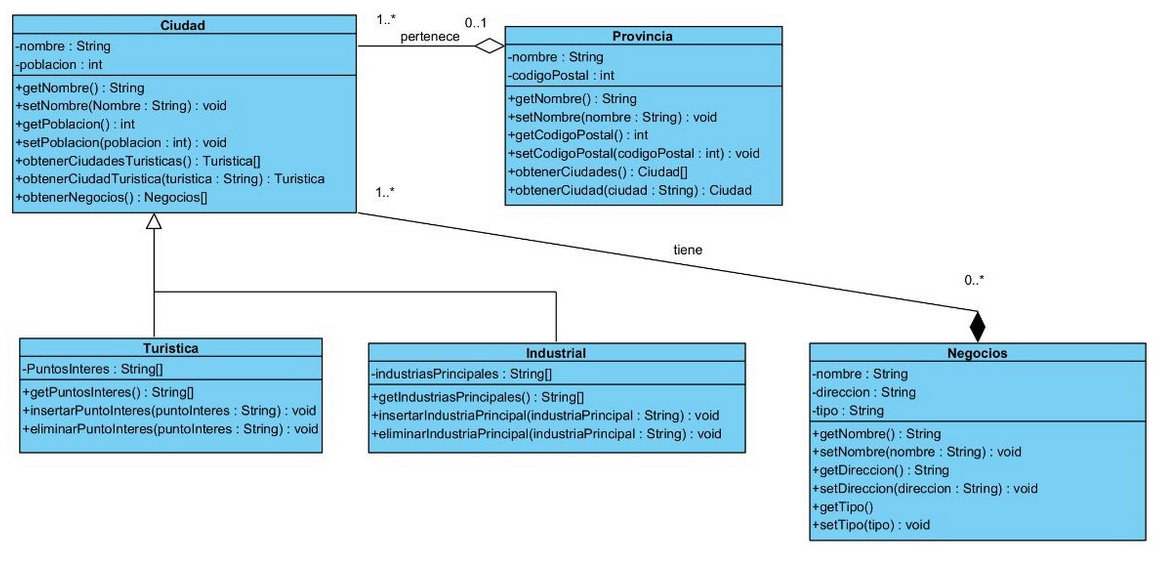
\includegraphics[scale=0.30]{diagrama-clases.png}
    \caption{Diagrama de Clases}
\end{figure}

\subsubsection{Solución}
En este primer ejercicio, hemos creado un proyecto en Visual Paradigm. El proyecto se incluye dentro de los archivos entregados, pero a continuación se muestra la diagrama creado en Visual Paradigm. Se han  redistribuido un poco las clases para que quede más ordenado.

\begin{figure}[H]
    \centering
    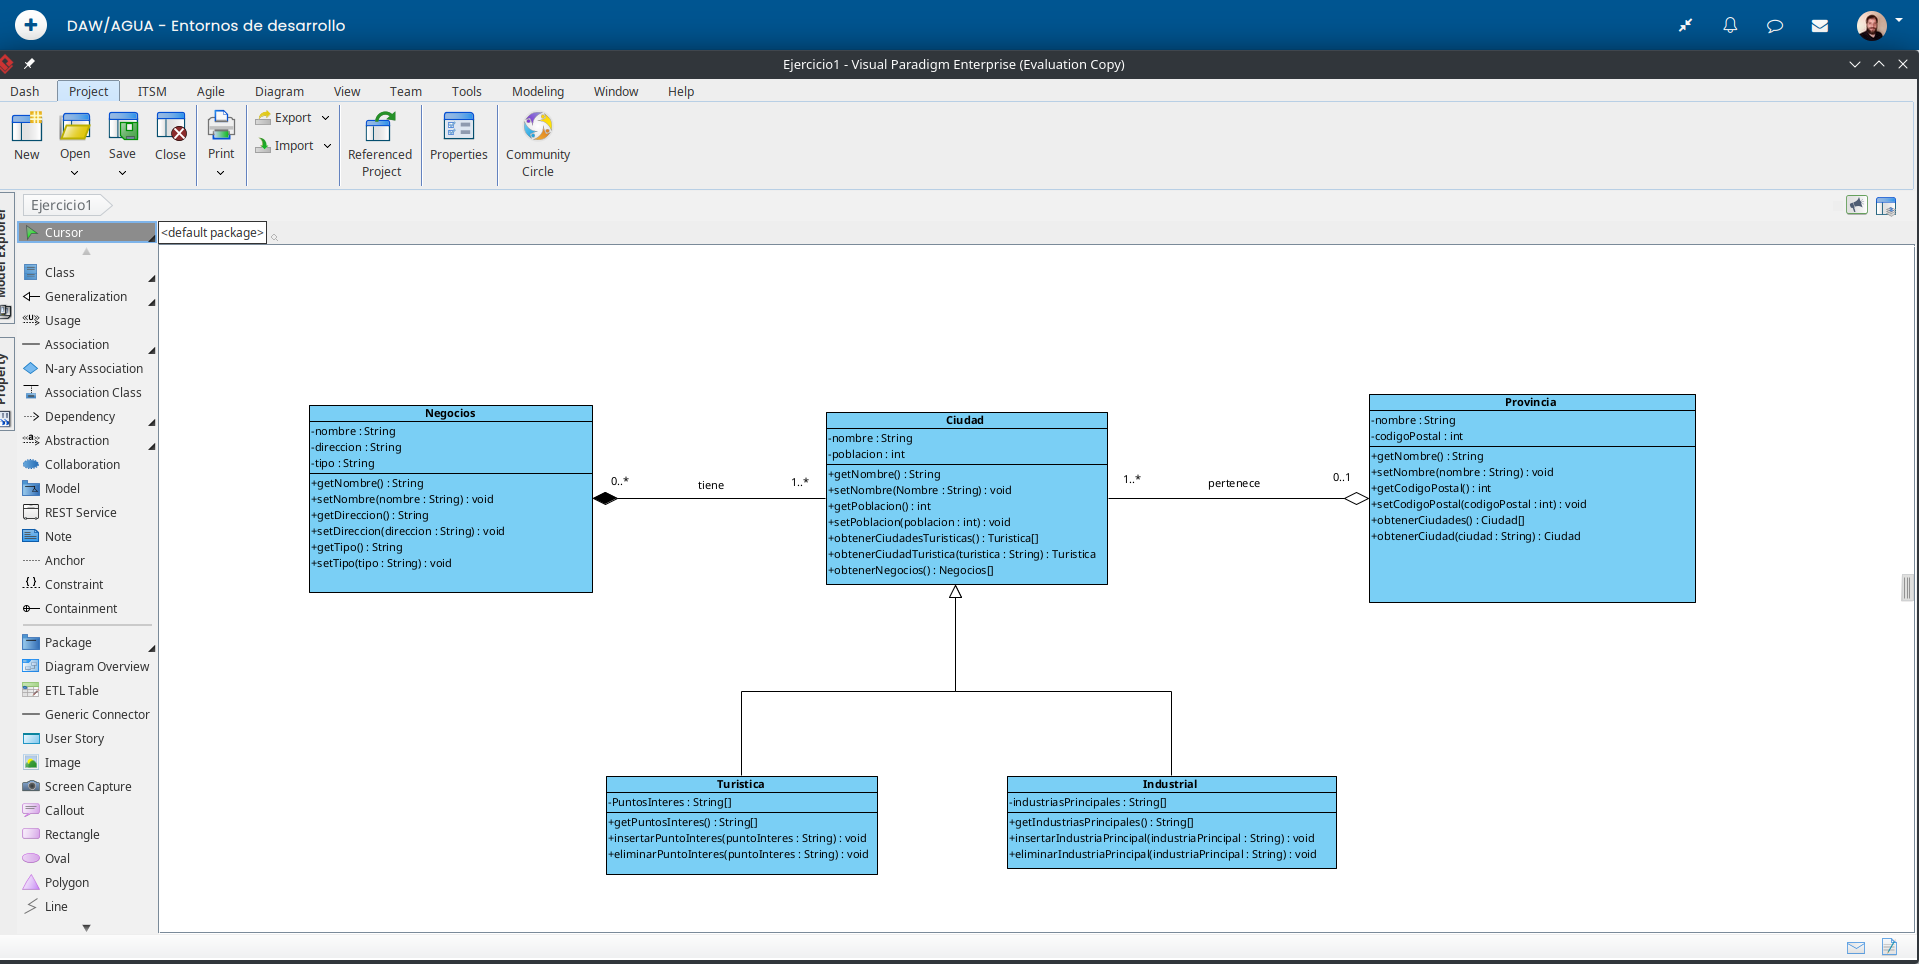
\includegraphics[scale=0.20]{diagrama-vp.png}
    \caption{Diagrama creado en Visual Paradigm}
\end{figure}

\subsection{Ejercicio 2}

\subsubsection{Enunciado}
Importación del proyecto VP-UML en un proyecto de NetBeans. (Breve descripción de los pasos a seguir incluyendo capturas de pantalla).

\subsubsection{Solución}
En este ejercicio vamos a importar el proyecto que hemos creado en el anterior en VP a Netbeans. Para ellos, vamos a seguir una serie de pasos los cuales describimos a continuación.

\begin{enumerate}
    \item En primer lugar, tenemos que realizar la \textbf{integración} de Visual Paradigm en Netbeans. Para ello abrimos VP y pulsamos en la opción del menú superior ``\textit{Windows}, lo cual nos mostrará diversas opciones  en la barra superior. Tenemos que pulsar en la opción ``\textit{Integration} y dentro de las dos opciones que se nos despliegan, pulsar en ``\textit{IDE Integration...}, como podemos ver en la siguiente captura.

    \begin{figure}[H]
        \centering
        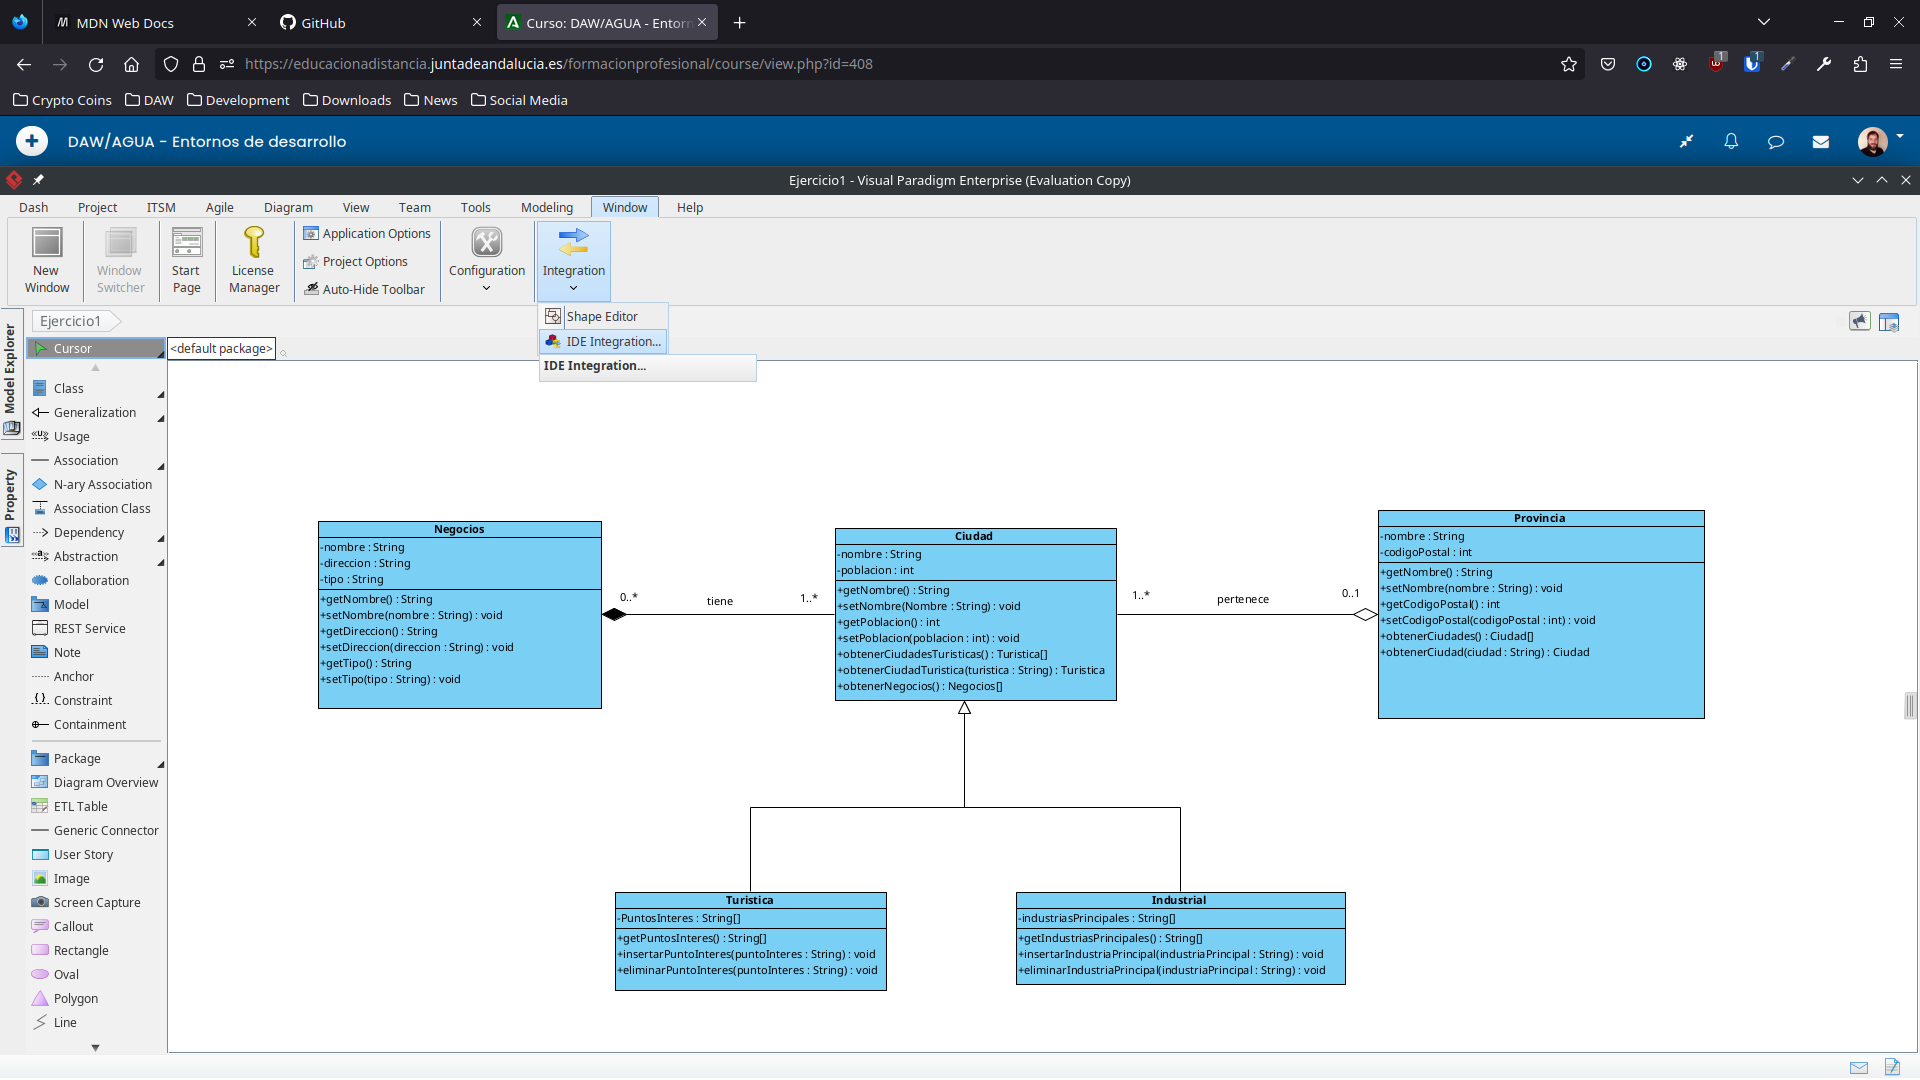
\includegraphics[scale=0.20]{vp-netbeans-1.png}
        \caption{Integración de VP en Netbeans (1)}
    \end{figure}

    Una vez pulsada en la opción anterior, se nos mostrará una ventana donde deberemos seleccionar el IDE en el que queremos realizar la integración, en nuestro caso, seleccionaremos \textbf{Netbeans} y pulsamos en ``\textit{Next}''.

     \begin{figure}[H]
        \centering
        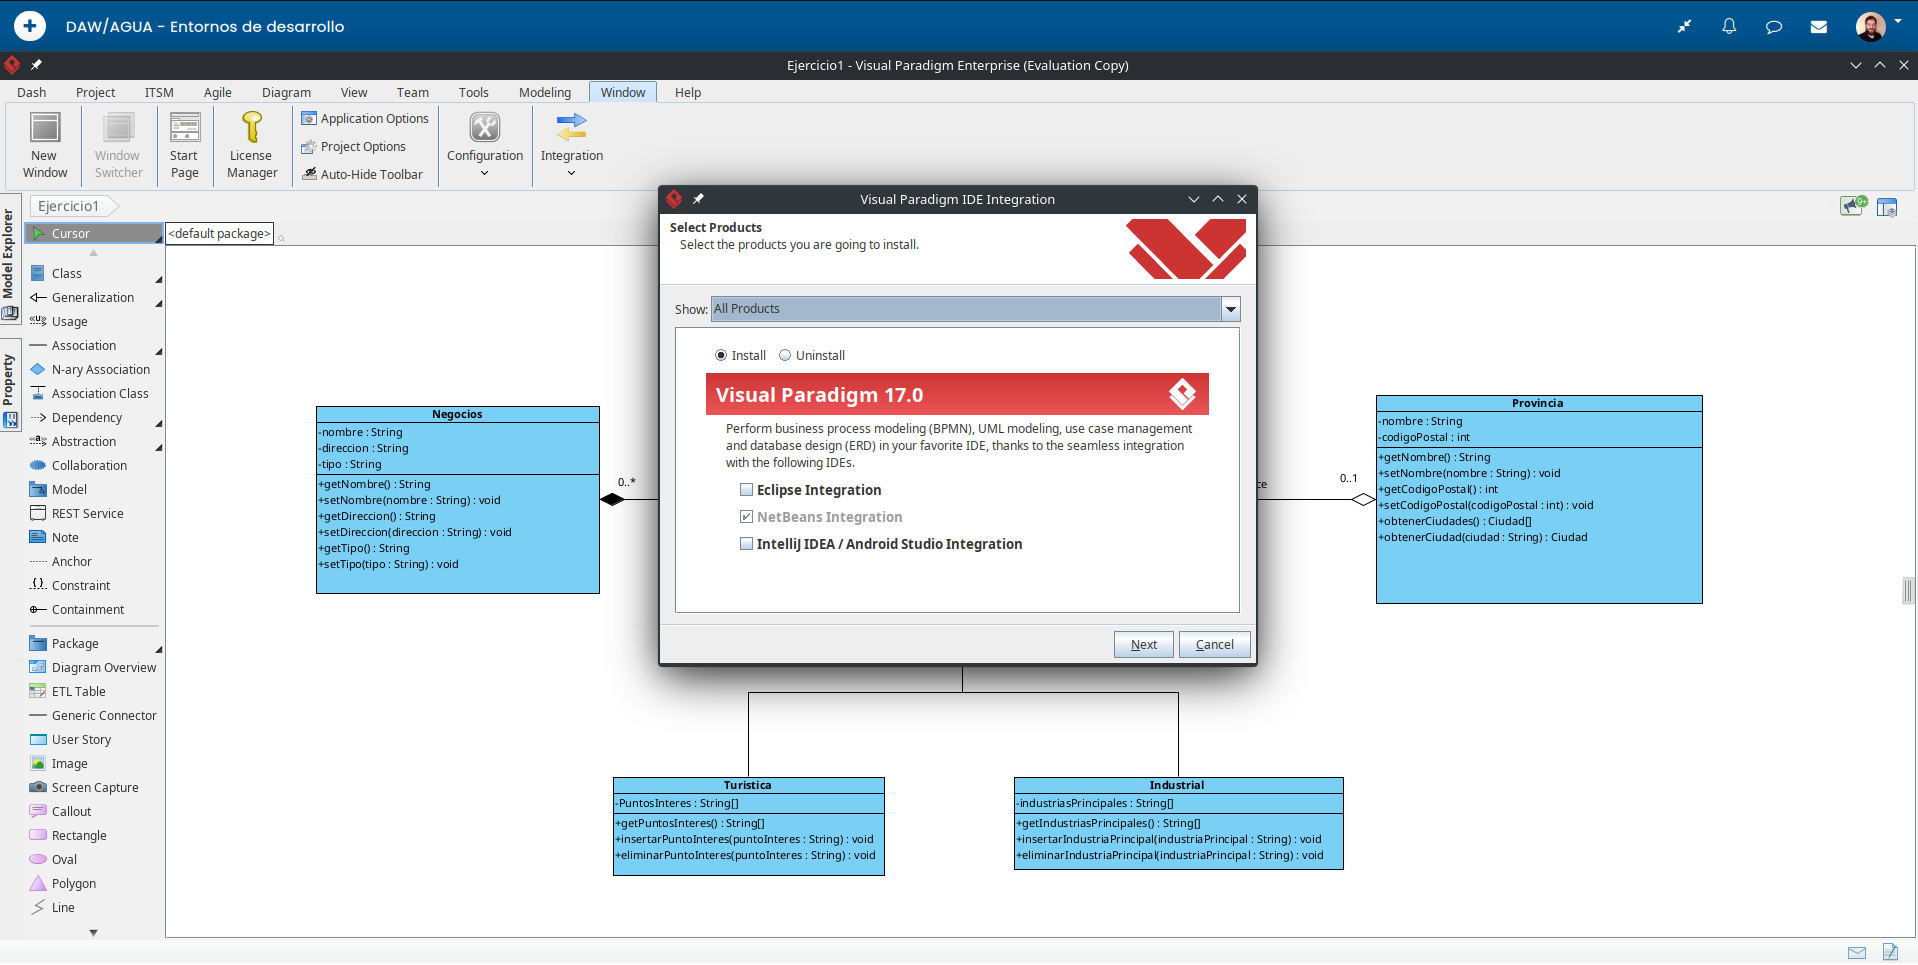
\includegraphics[scale=0.20]{vp-netbeans-2.png}
        \caption{Integración de VP en Netbeans (2)}
    \end{figure}

    Una vez hecho esto, se copiarán todos los archivos necesarios en el directorio de instalación de Netbeans y la integración se habrá realizado con éxito.


    \item El siguiente paso deberemos darlo en Netbeans. En primer lugar abrimos \textbf{Netbeans} y \textbf{creamos un proyecto}, ya que para poder usar VP en Netbeans debemos hacerlo sobre un proyecto que hayamos creado. Para ello, pulsamos en la opción ``\textit{File}-->\textit{New project}'' del menú de la barra superior de Netbeans, lo que nos abrirá la ventana para la creación del nuevo proyecto.

    \begin{figure}[H]
        \centering
        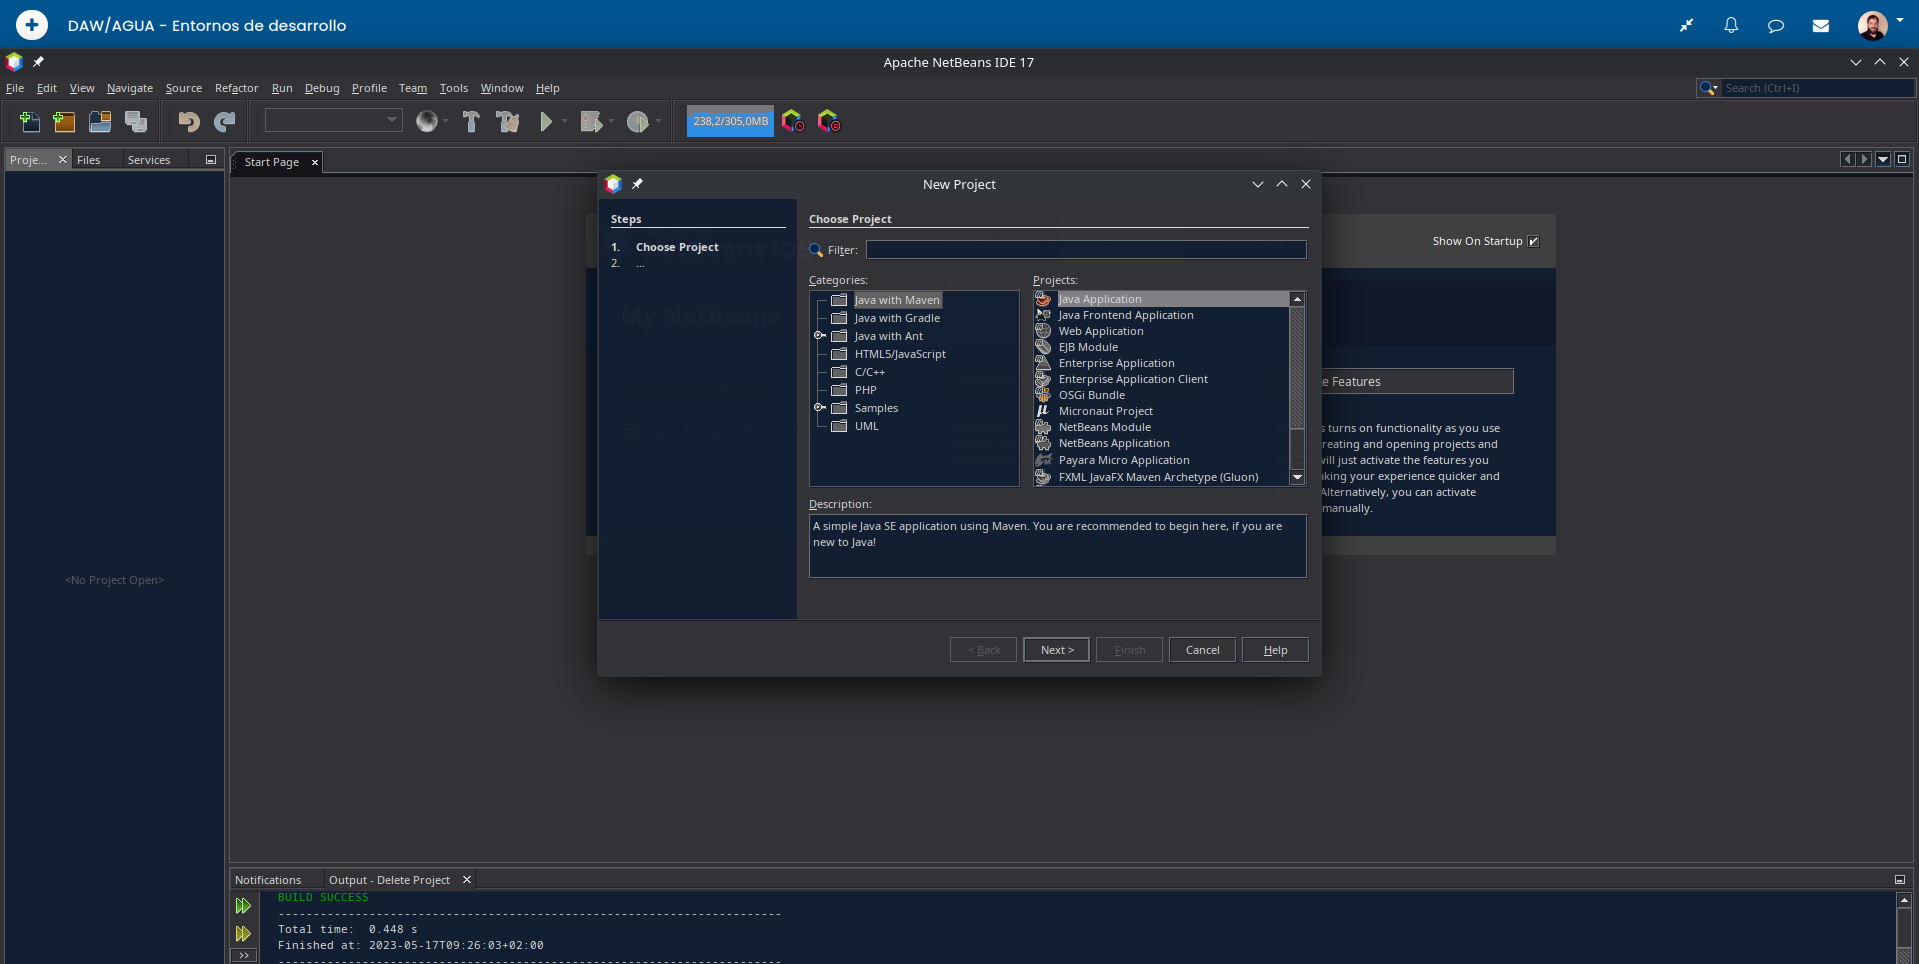
\includegraphics[scale=0.23]{vp-netbeans-3.png}
        \caption{Creación de proyecto en Netbeans (1)}
    \end{figure}

    En la ventana que se nos abre, seleccionamos la opción ``\textit{Java Aplication}'' para crear una aplicación java y pulsamos en ``\textit{Next}'', lo que nos mostrará la siguiente ventana donde podemos incluir información sobre el proyecto, como su nombre, la carpeta donde se va a almacenar, etc... Nosotros hemos nombrado el proyecto según las especificaciones de la tarea con nuestro nombre y apellidos.

    \begin{figure}[H]
        \centering
        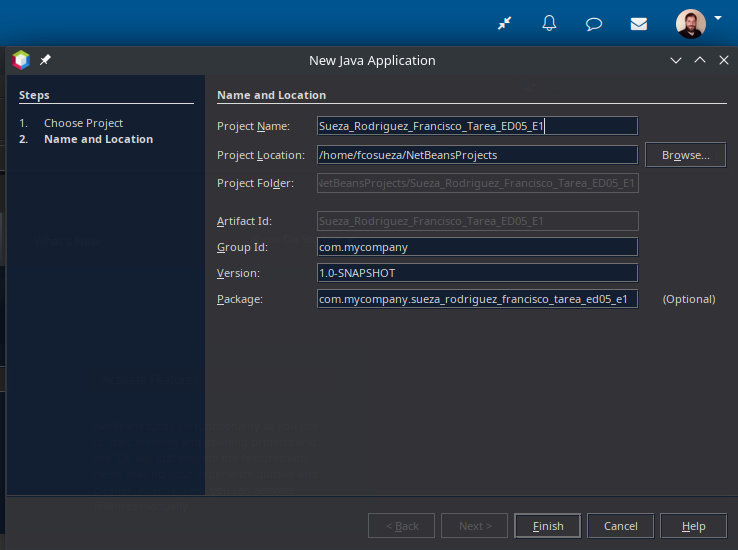
\includegraphics[scale=0.45]{vp-netbeans-4.png}
        \caption{Creación de proyecto en Netbeans (2)}
    \end{figure}

    Una vez introducidos los datos, el proyectos se creará con los archivos por defecto y se nos abrirá automáticamente el fichero principal, donde se encuentra el método main.

    \item A continuación, debemos \textbf{inicializar VP en Netbeans}. Para ello, pulsamos con el botón derecho sobre el proyecto que acabamos de crear y pulsamos en la opción ``\textit{Open Visual Paradigm Enterprise}.

    \begin{figure}[H]
        \centering
        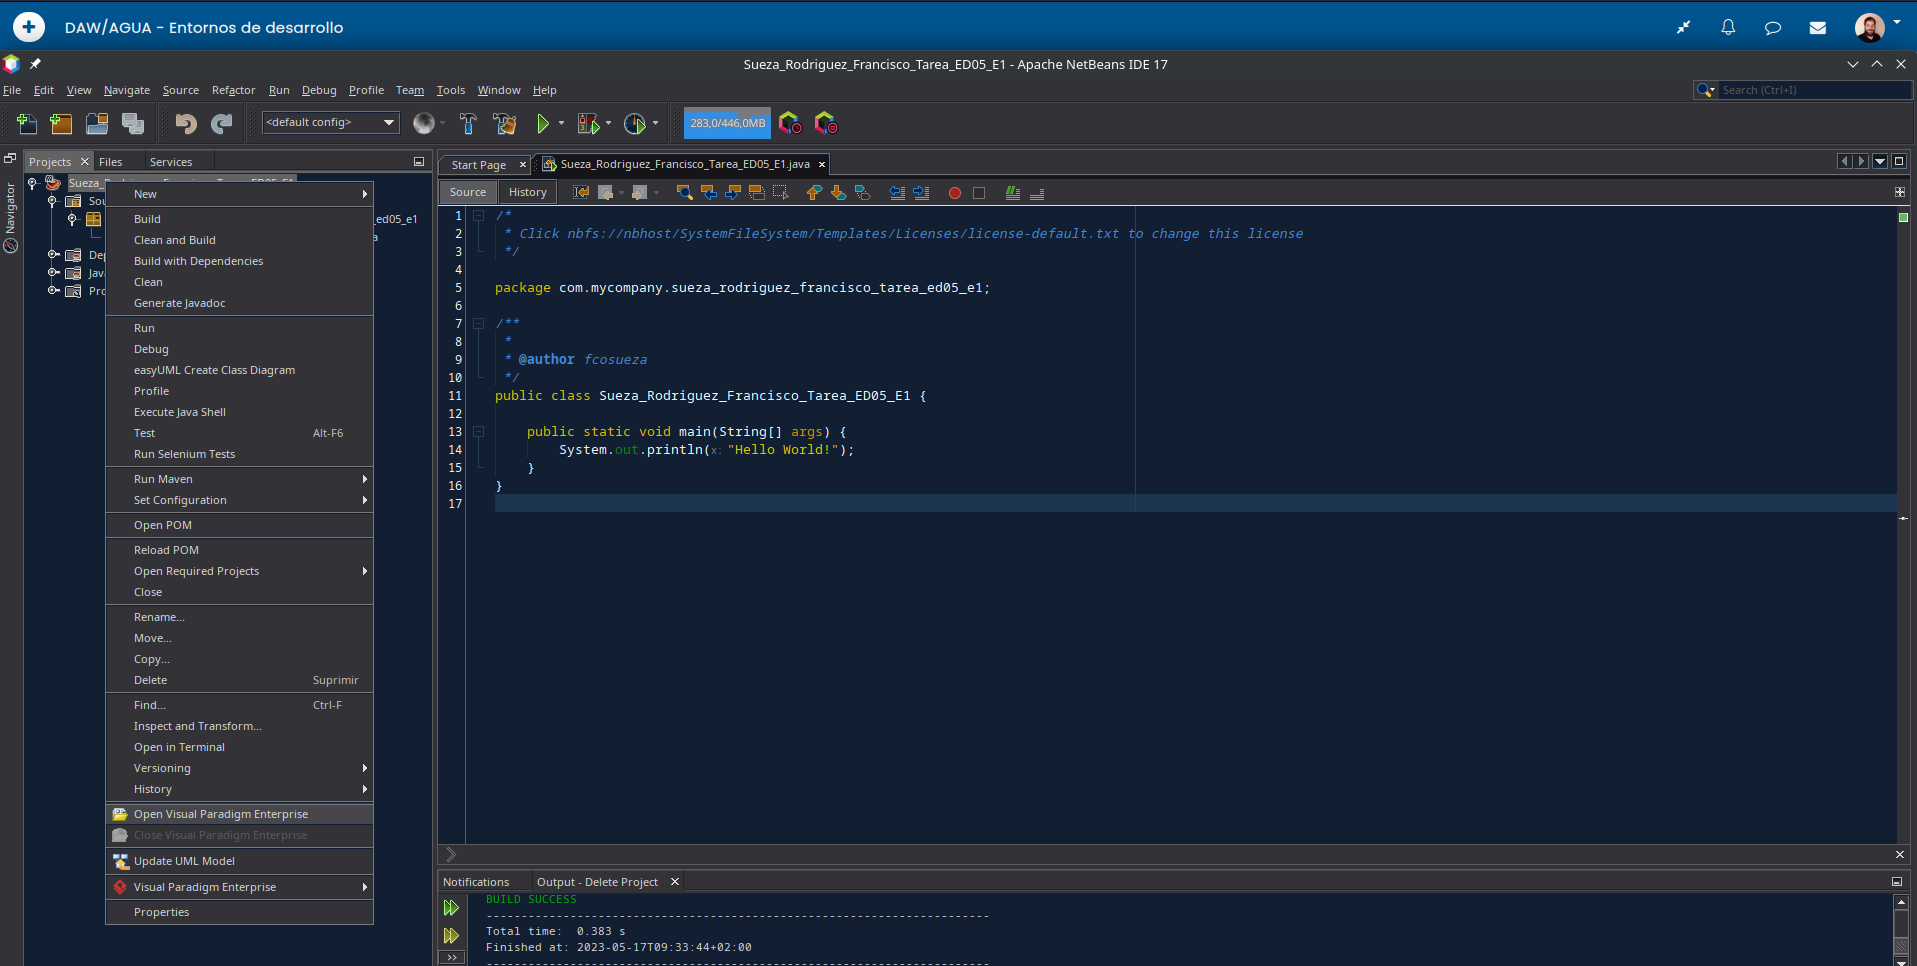
\includegraphics[scale=0.23]{vp-netbeans-5.png}
        \caption{Inicialización de VP en Netbeans (1)}
    \end{figure}

    Una vez pulsado, \textbf{comenzará la carga de Visual Paradigm}, lo que se nos mostrará con la ventana de carga por defecto de esta aplicación. Este proceso puede tardar más o menos, ya dependiendo de las especificaciones de hardware de tu dispositivos o  del SO donde lo estés realizando.

    Una vez realizada la carga de VP, nos aparecerán nuevas opciones, en la barra superior de Netbeans, para la creación de los diferentes tipos de diagramas, así como nuevas pestañas encima del proyecto con diferentes opciones, etc.., como podemos ver en la siguiente captura de pantalla.

    \begin{figure}[H]
        \centering
        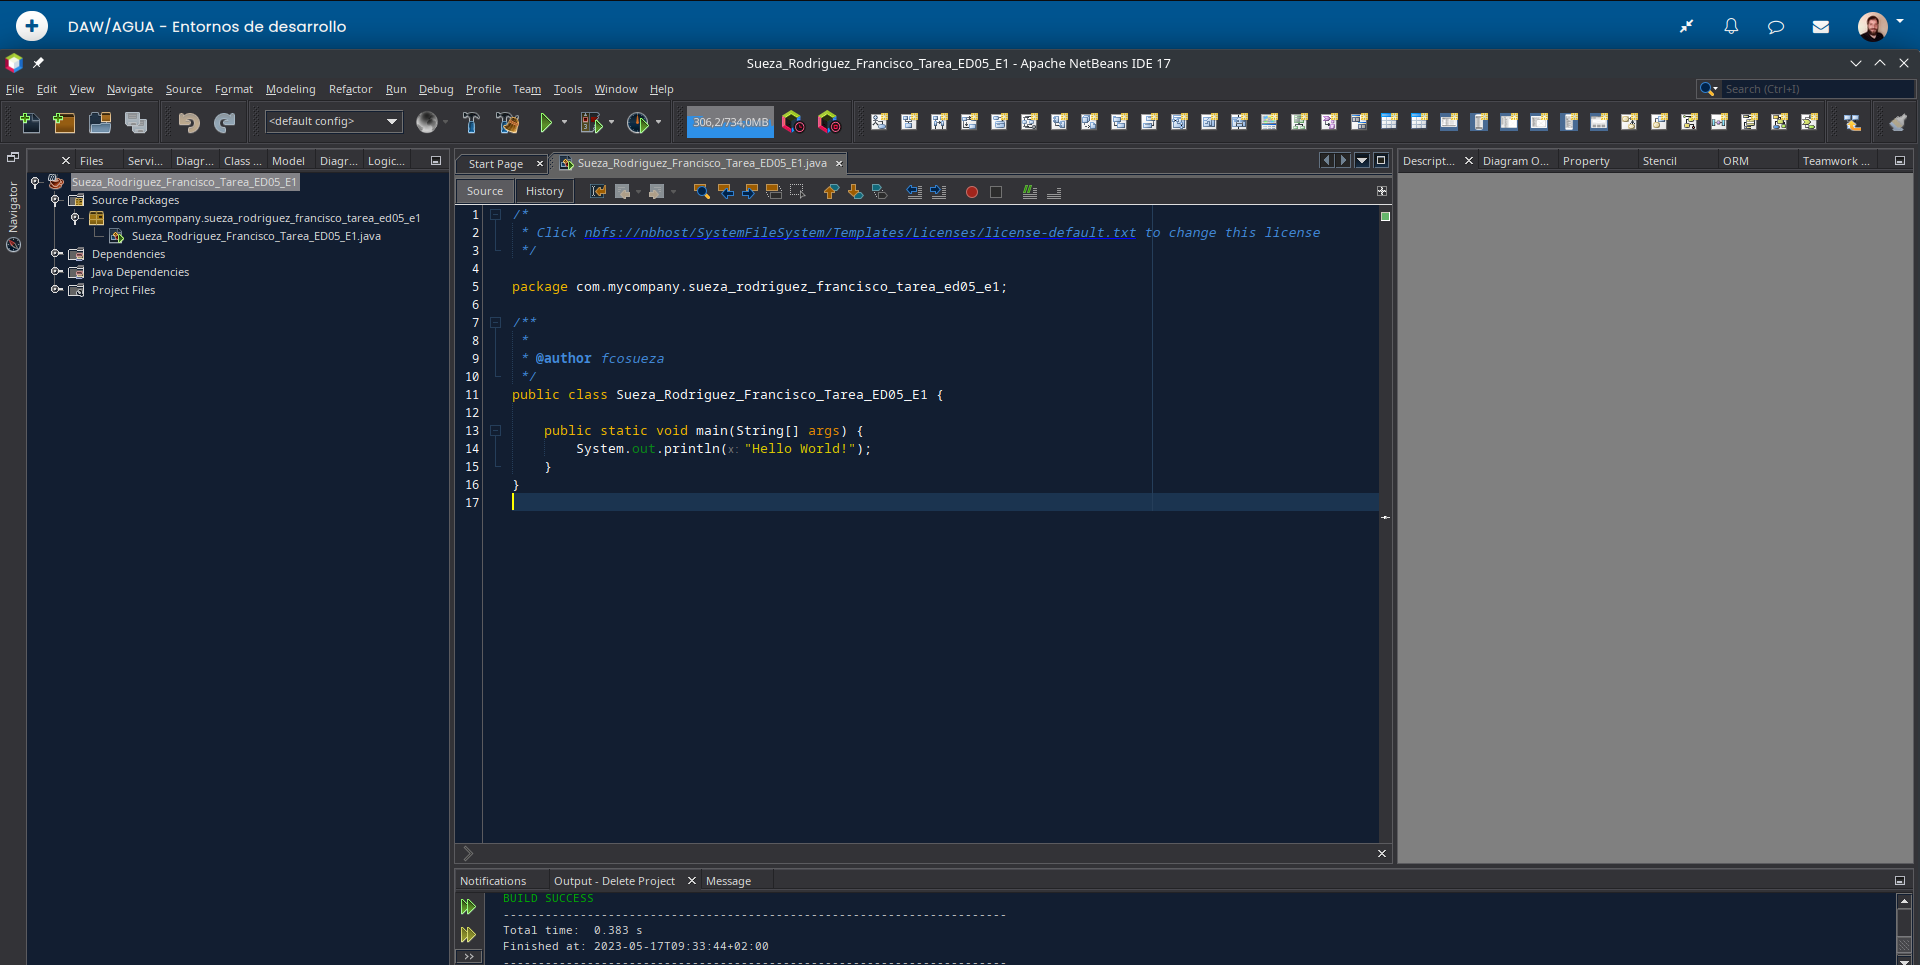
\includegraphics[scale=0.23]{vp-netbeans-6.png}
        \caption{Inicialización de VP en Netbeans (2)}
    \end{figure}

    \item El siguiente paso será \textbf{importar el proyecto de VP}. Para ello, tenemos que pulsar el la opción ``\textit{File}'' del menú superior y dentro de este en las opciones ``\textit{Visual Paradigm Enterprise Import}-->\textit{UML Model}'', como vemos en la siguiente imagen.

    \begin{figure}[H]
        \centering
        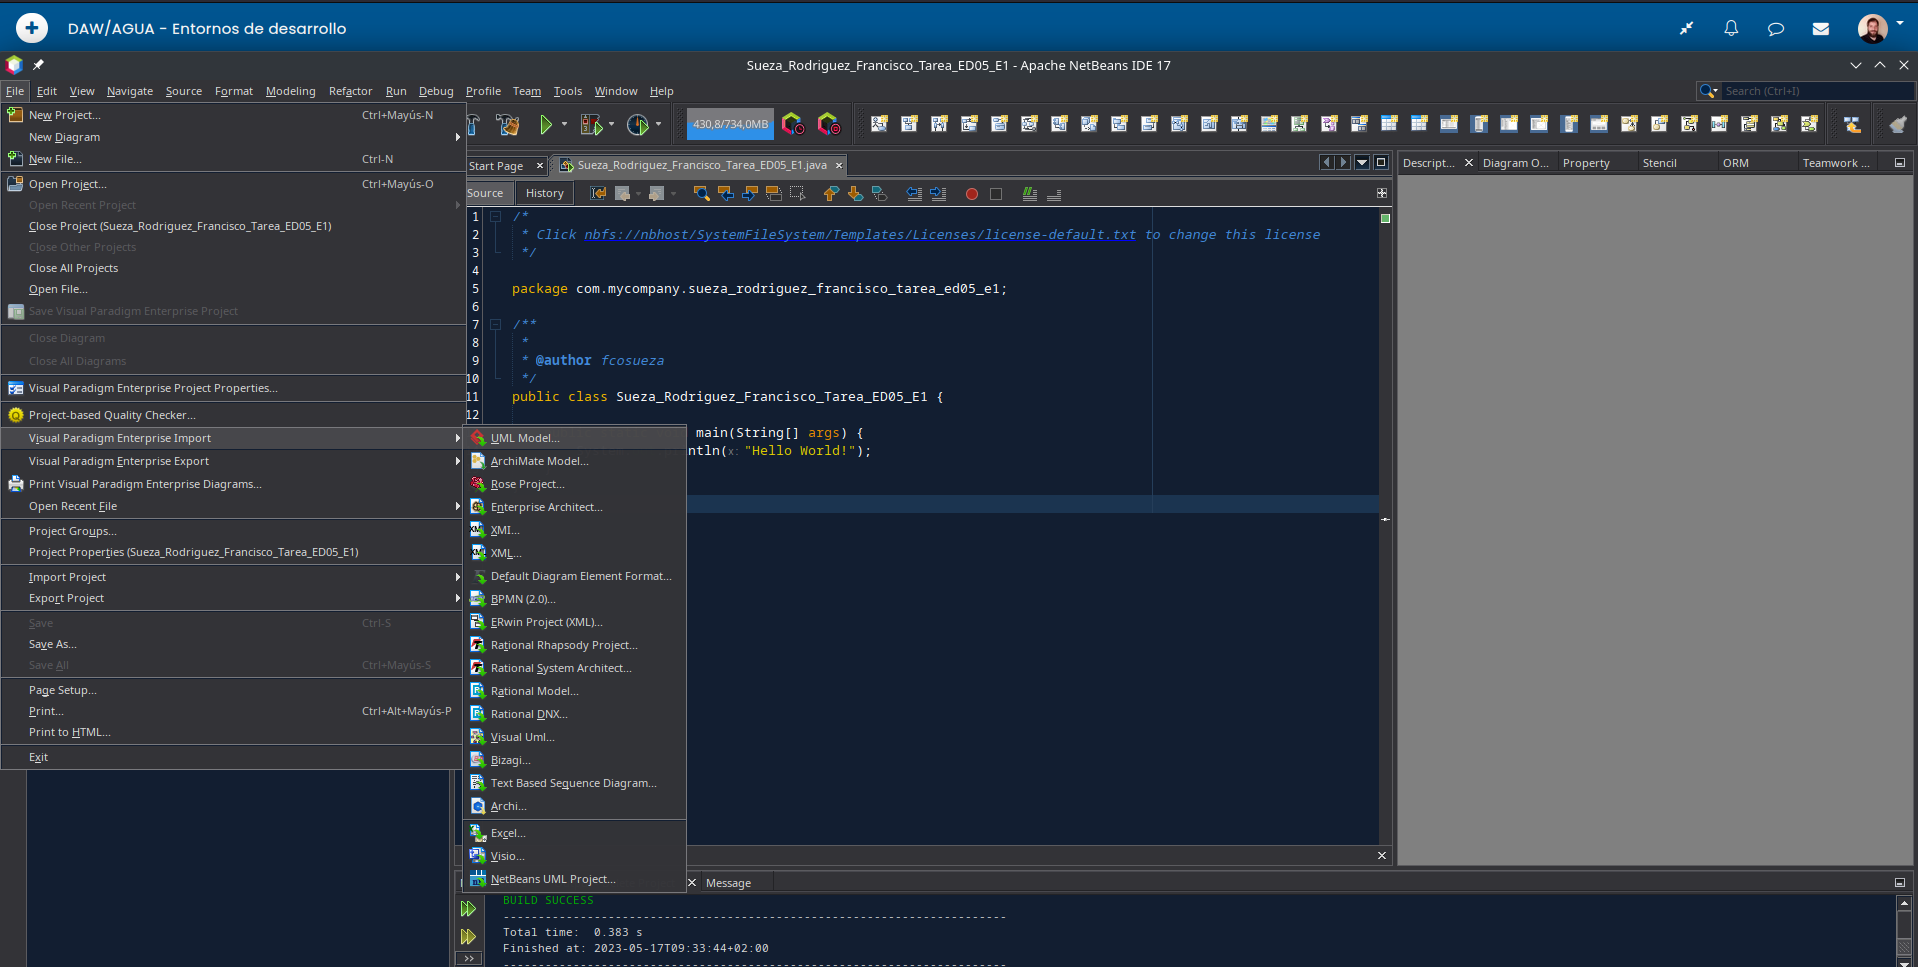
\includegraphics[scale=0.25]{vp-netbeans-7.png}
        \caption{Importación del proyecto VP (1)}
    \end{figure}

    Esto nos mostrará una ventana donde podemos \textbf{seleccionar el archivo} que queremos importar. Seleccionamos el archivo de nuestro proyecto de VP y pulsamos el ``\textit{Open}''.

    \begin{figure}[H]
        \centering
        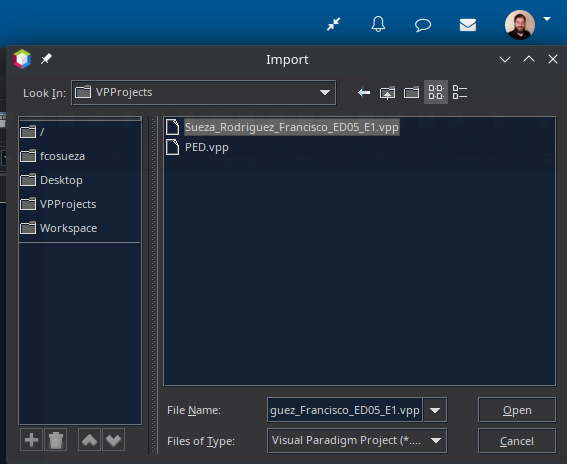
\includegraphics[scale=0.50]{vp-netbeans-8.png}
        \caption{Importación del proyecto VP (2)}
    \end{figure}

    \item Una vez realizado el paso anterior, el proyecto se habrá \textbf{importado correctamente}, pero aún no veremos el proyecto en la pantalla de Netbeans.

    Para que podamos ver el proyecto, debemos seleccionar la pestaña ``\textit{Diagramas}'', que nos habrá aparecido encima de la ventana del proyecto cuando cargamos VP. En esta pestaña, deberemos seleccionar la opción ``\textit{Class Diagram}'' y hacer doble-click sobre el nombre de nuestro proyecto VP.

    Hay que tener en cuenta que el nombre que aparecerá no es el del archivo de nuestro proyecto, sino el nombre que le hayamos puesto al proyecto dentro de las propiedades en VP.

    Una vez hecho esto, nuestro proyecto de VP se mostrará en la ventana principal de Netbeans, como vemos en la siguiente captura.

    \begin{figure}[H]
        \centering
        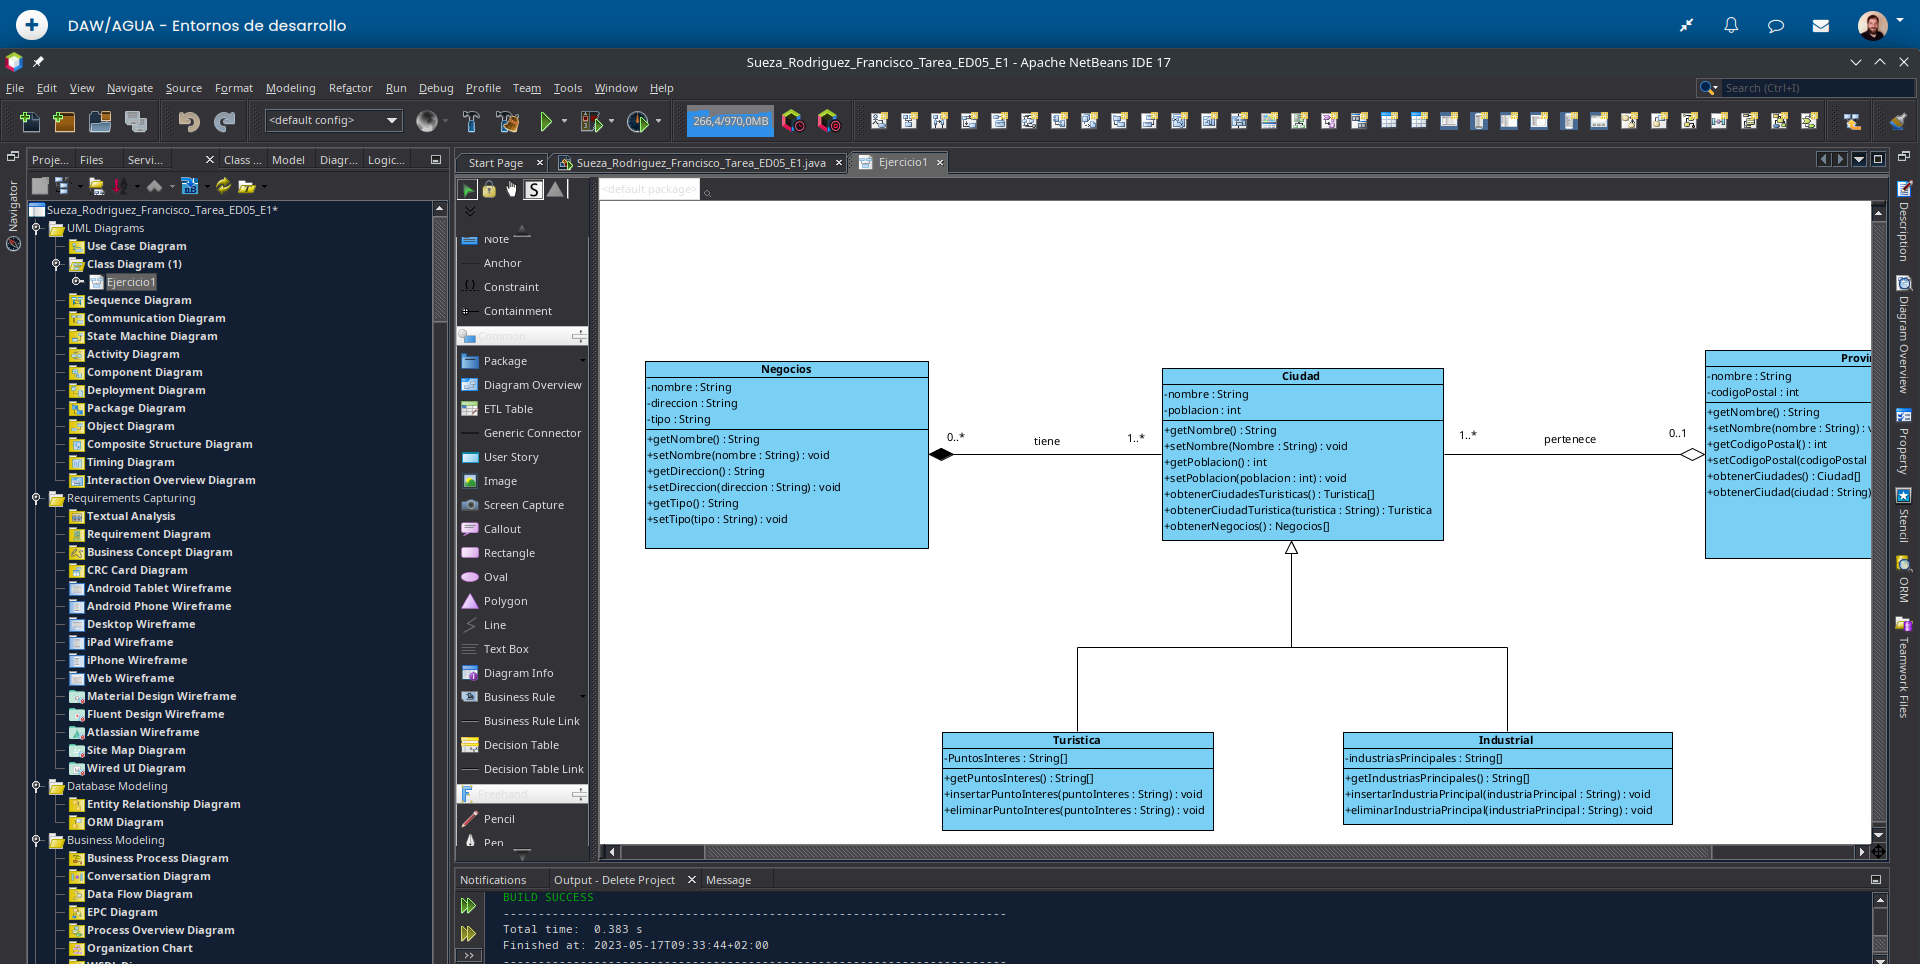
\includegraphics[scale=0.25]{vp-netbeans-9.png}
        \caption{Proyecto VP cargado en Netbeans}
    \end{figure}
\end{enumerate}

\subsection{Ejercicio 3}

\subsubsection{Enunciado}
Generación del código a partir del diagrama de clases realizado.

\subsubsection{Solución}
En este ejercicio vamos a generar el código Java a partir del diagrama que hemos creado. Podemos hacerlo desde Visual Paradigm o desde Netbeans. Para que se continúe con el ejercicio anterior, y ya que no se especifica en el enunciado del ejercicio de que forma hacerlo, nosotros lo vamos a hacer desde \textbf{Netbeans}, ya que así, además, tendremos el proyecto Java generado cargado directamente en nuestro IDE.

Para generar el código, partiendo de la pestaña ``\textit{Diagramas}'' que se nos creo encima de la ventana del proyecto al cargar VP en Netbeans, pulsamos en el \textbf{icono azul} justo encima de la ventana donde seleccionamos los diagramas, como vemos en la siguiente imagen, y seleccionamos la opción ``\textit{Update code}''.

\begin{figure}[H]
    \centering
    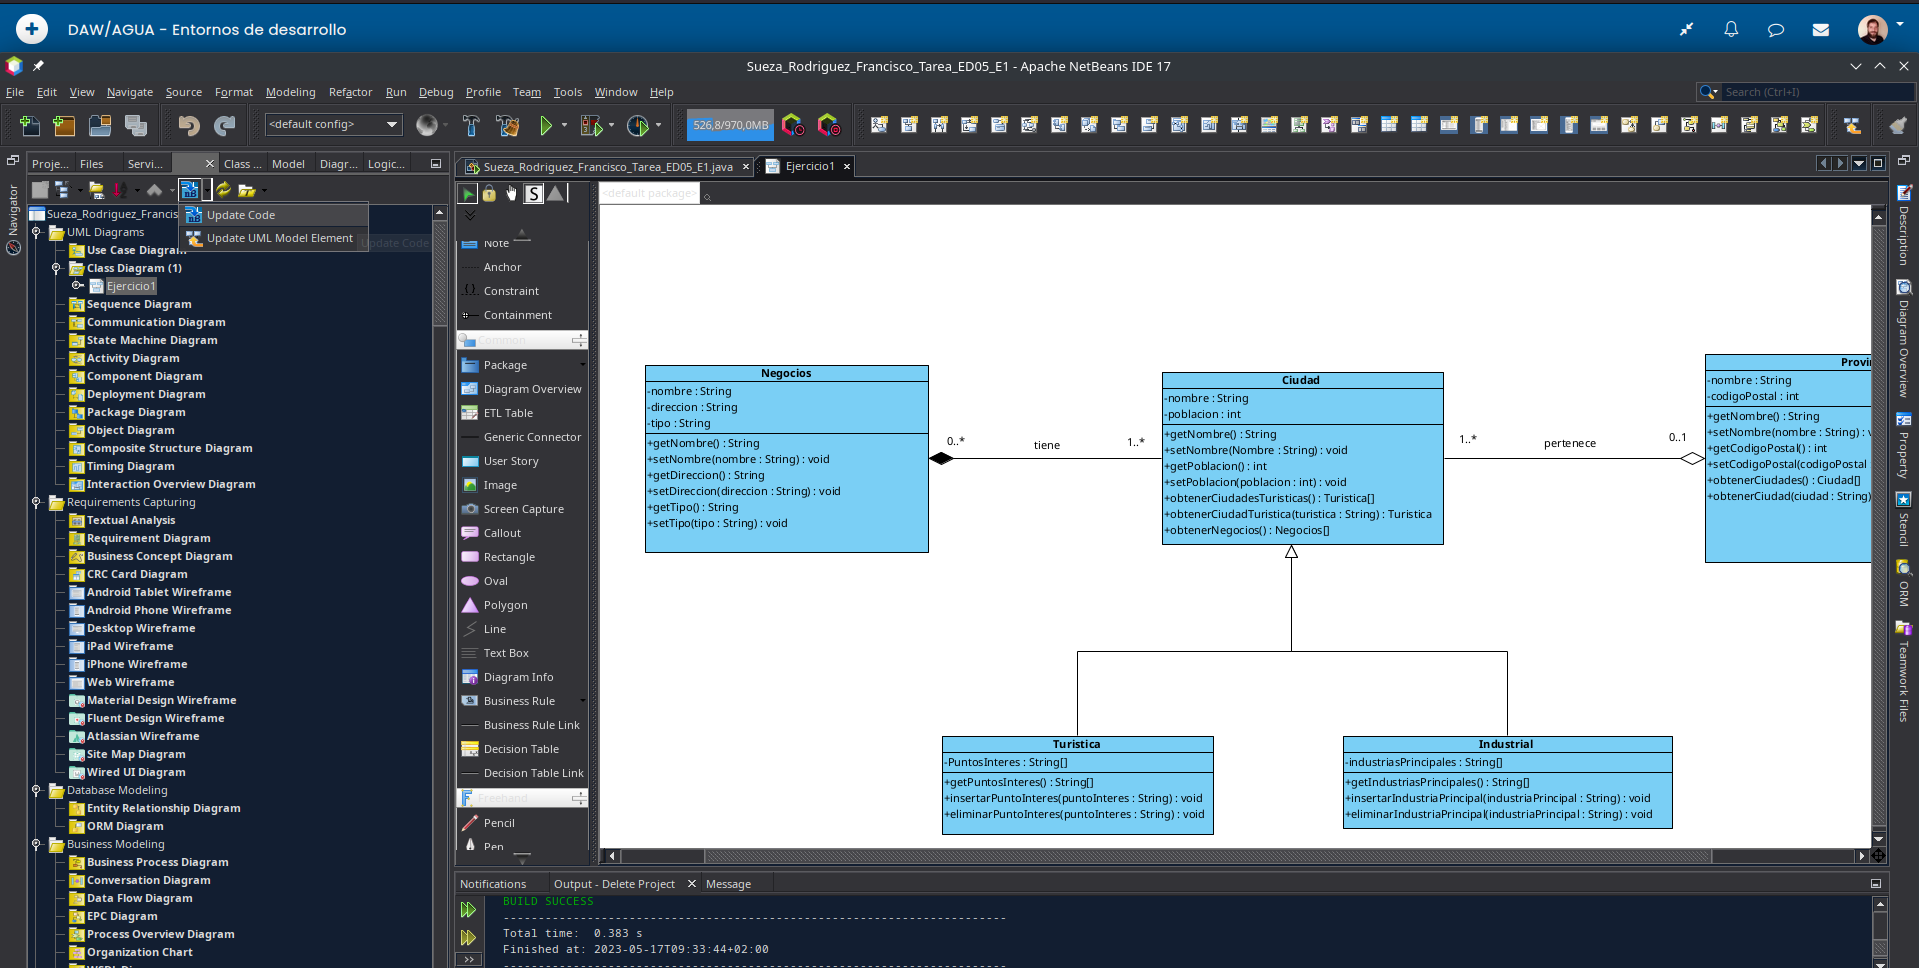
\includegraphics[scale=0.23]{code-gen-1.png}
    \caption{Generación de código a partir del proyecto VP (1)}
\end{figure}

Es posible que nos muestre algún error, si hay algo que no esta bien en el diagrama, como puede ser un tipo de retorno erróneo en algún método. Si fuera el caso, corregimos el error, y volvemos a pulsar en esta opción. Esto, generará un conjunto de clases acordes al diagrama de clases.  Es posible que algunas relaciones no se hayan traducido, por lo que tendremos que hacerlo de forma manual.

\begin{figure}[H]
    \centering
    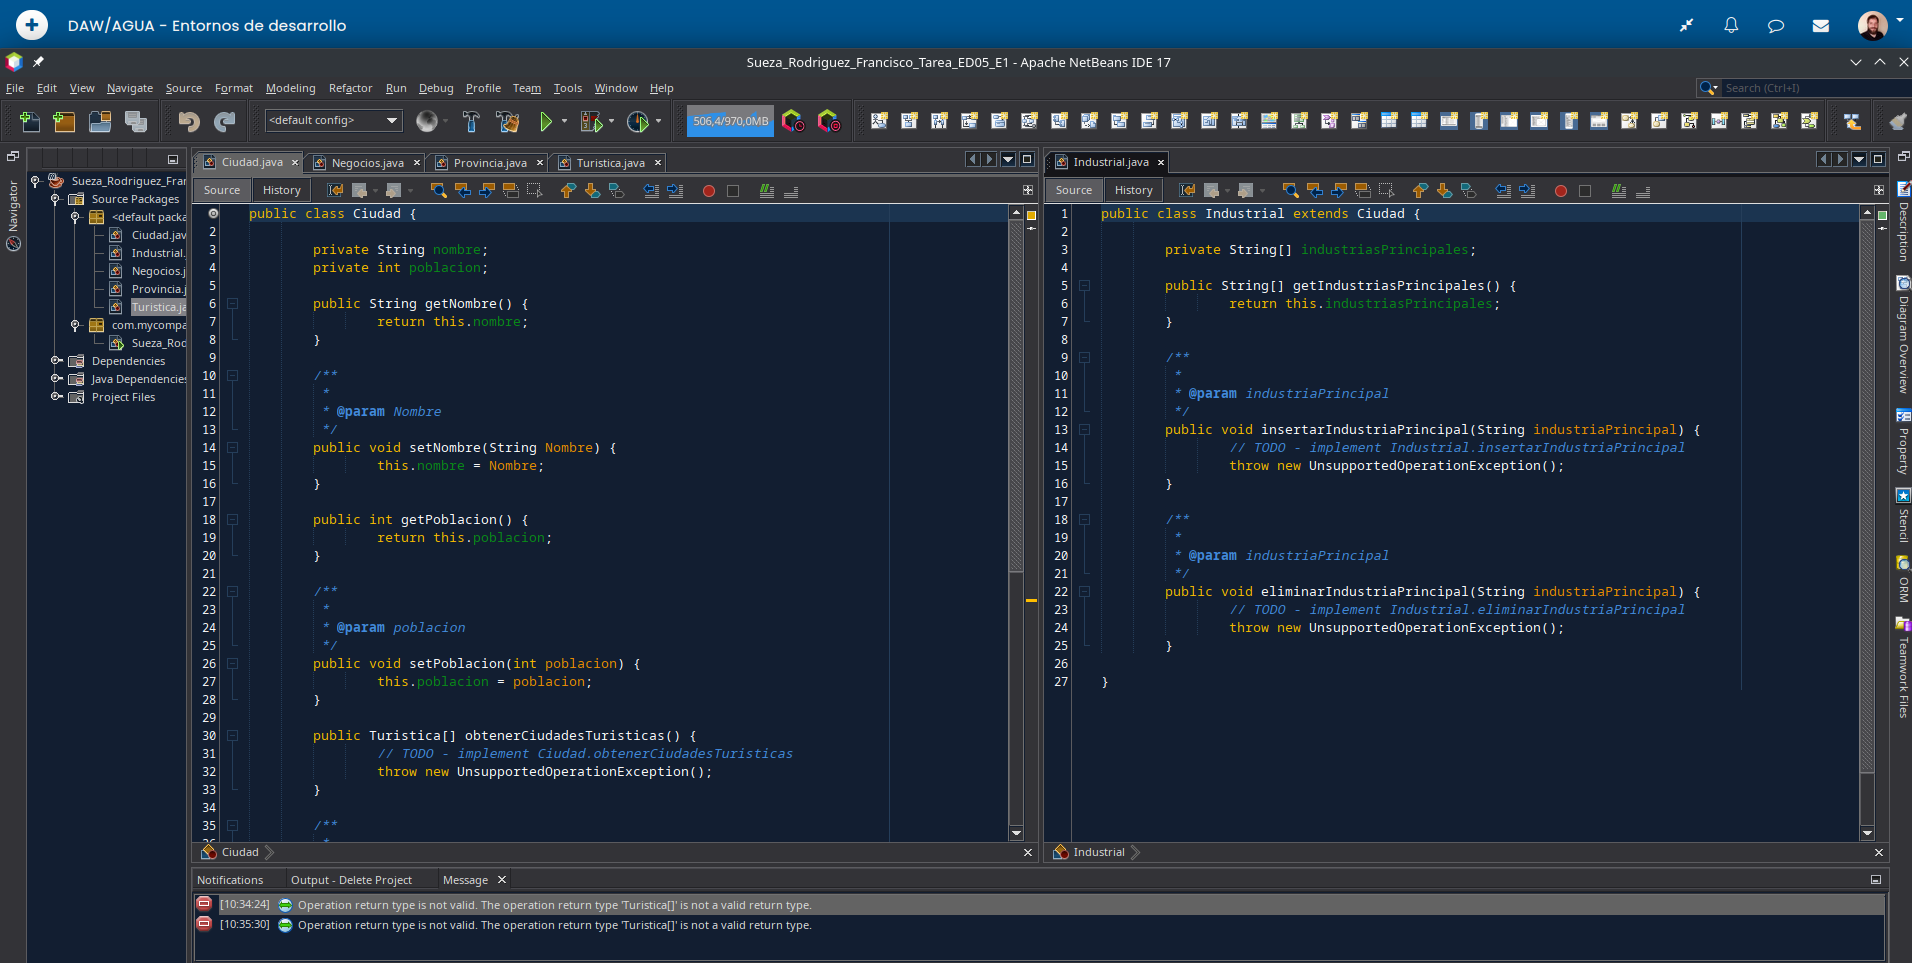
\includegraphics[scale=0.20]{code-gen-2.png}
    \caption{Generación de código a partir del proyecto VP (2)}
\end{figure}

\subsection{Ejercicio 4}

\subsubsection{Enunciado}
Mediante el proceso de ingeniería inversa, genera el diagrama de clases a partir del siguiente \href{https://www.juntadeandalucia.es/educacion/gestionafp/datos/tareas/DAM/ED_22878/2022-23/DAM_ED_5_2022-23_Individual__968293/ingenieriaInversa_XXX2223.zip}{proyecto Java}. Si al realizar este proceso faltan relaciones, tendrás que establecerlas a mano.  (No olvides refactorizar y cambiar XXX por tus datos para cumplir el requisito de corrección). Puedes hacer uso del plugin EasyUML (enlaces en la sección Información de interés).

\subsubsection{Solución}
En este ejercicio vamos a realizar el proceso de ingeniería inversa con el proyecto Java que se nos ha proporcionado. Para realizar este proceso, vamos a usar el plugin de Netbeans \textbf{EasyUML}, el cual podemos descargar desde \url{https://github.com/mgeee35/easyUML}.

Este proceso es bastante sencillo, y solo debemos seguir los siguientes pasos para llevarlo a cabo.

\begin{enumerate}
    \item En primer lugar, y teniendo ya el proyecto Java que se nos especifica cargado, debemos \textbf{crear otro proyecto}, de tipo \textbf{UML} en Netbeans. Para ello, pulsamos en la opción ``\textit{File}-->\textit{New Project...} del menú superior y seleccionamos UML como el tipo de proyecto a crear.

    \begin{figure}[H]
        \centering
        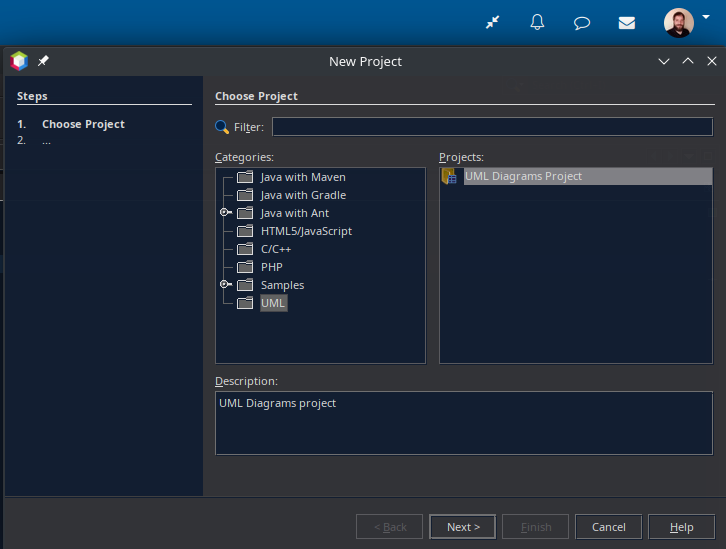
\includegraphics[scale=0.30]{inversa-1.png}
        \caption{Ingeniería Inversa: Creación proyecto UML}
    \end{figure}

    \item Una vez creado el proyecto UML, pulsamos sobre el \textbf{proyecto Java} con el botón derecho para que se despliegue el menú contextual y seleccionamos la opción ``\textit{easyUML Create Class Diagram}''.

    \begin{figure}[H]
        \centering
        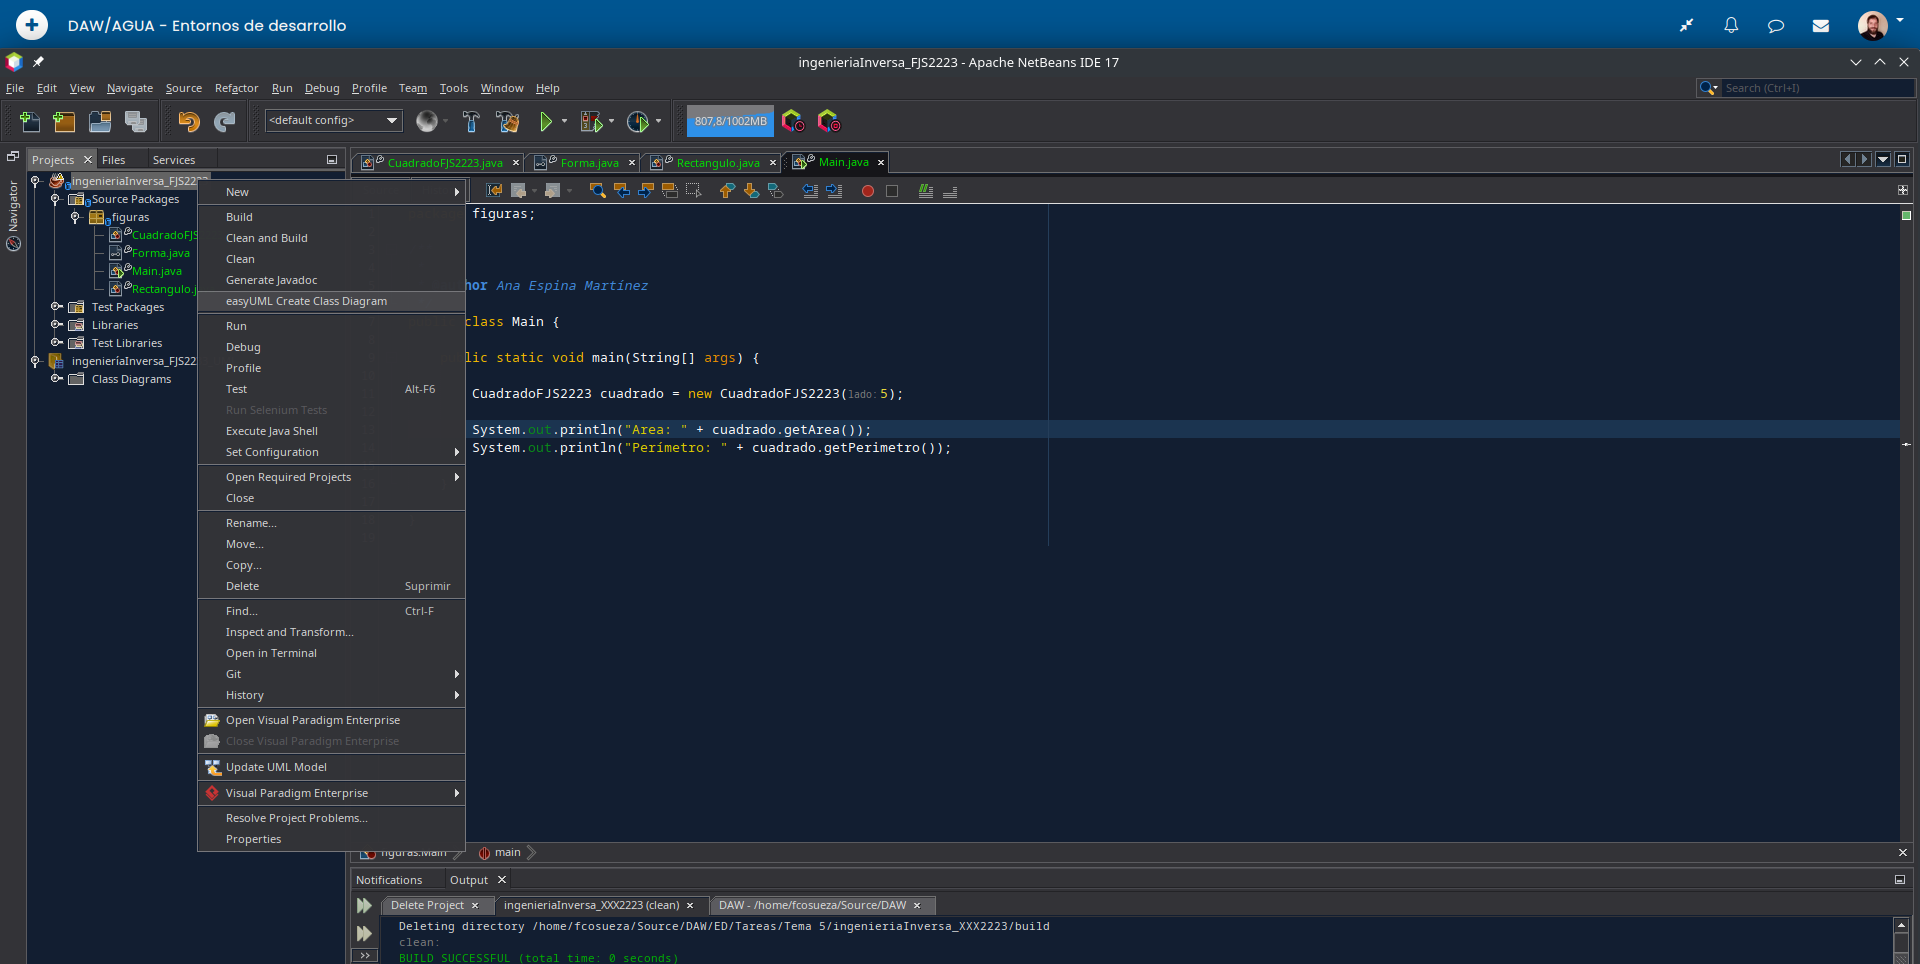
\includegraphics[scale=0.23]{inversa-2.png}
        \caption{Ingeniería Inversa: Seleccionar opción de easyUML}
    \end{figure}

    \item Esto nos mostrará una ventana donde debemos seleccionar el proyecto UML donde queremos que se generen los diagramas, que será el proyecto que hemos creado.

    \begin{figure}[H]
        \centering
        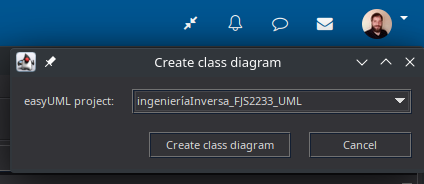
\includegraphics[scale=0.50]{inversa-3.png}
        \caption{Selección de proyecto UML}
    \end{figure}


    \item Tras el último paso, se nos habrá generado correctamente el \textbf{diagrama de clases} del proyecto Java. Podría ser que algunas relaciones falte en el diagrama generado, aunque no es nuestro caso, ya que se muestran las relaciones entre las clases correctamente, como podemos ver en la siguiente captura.

    \begin{figure}[H]
        \centering
        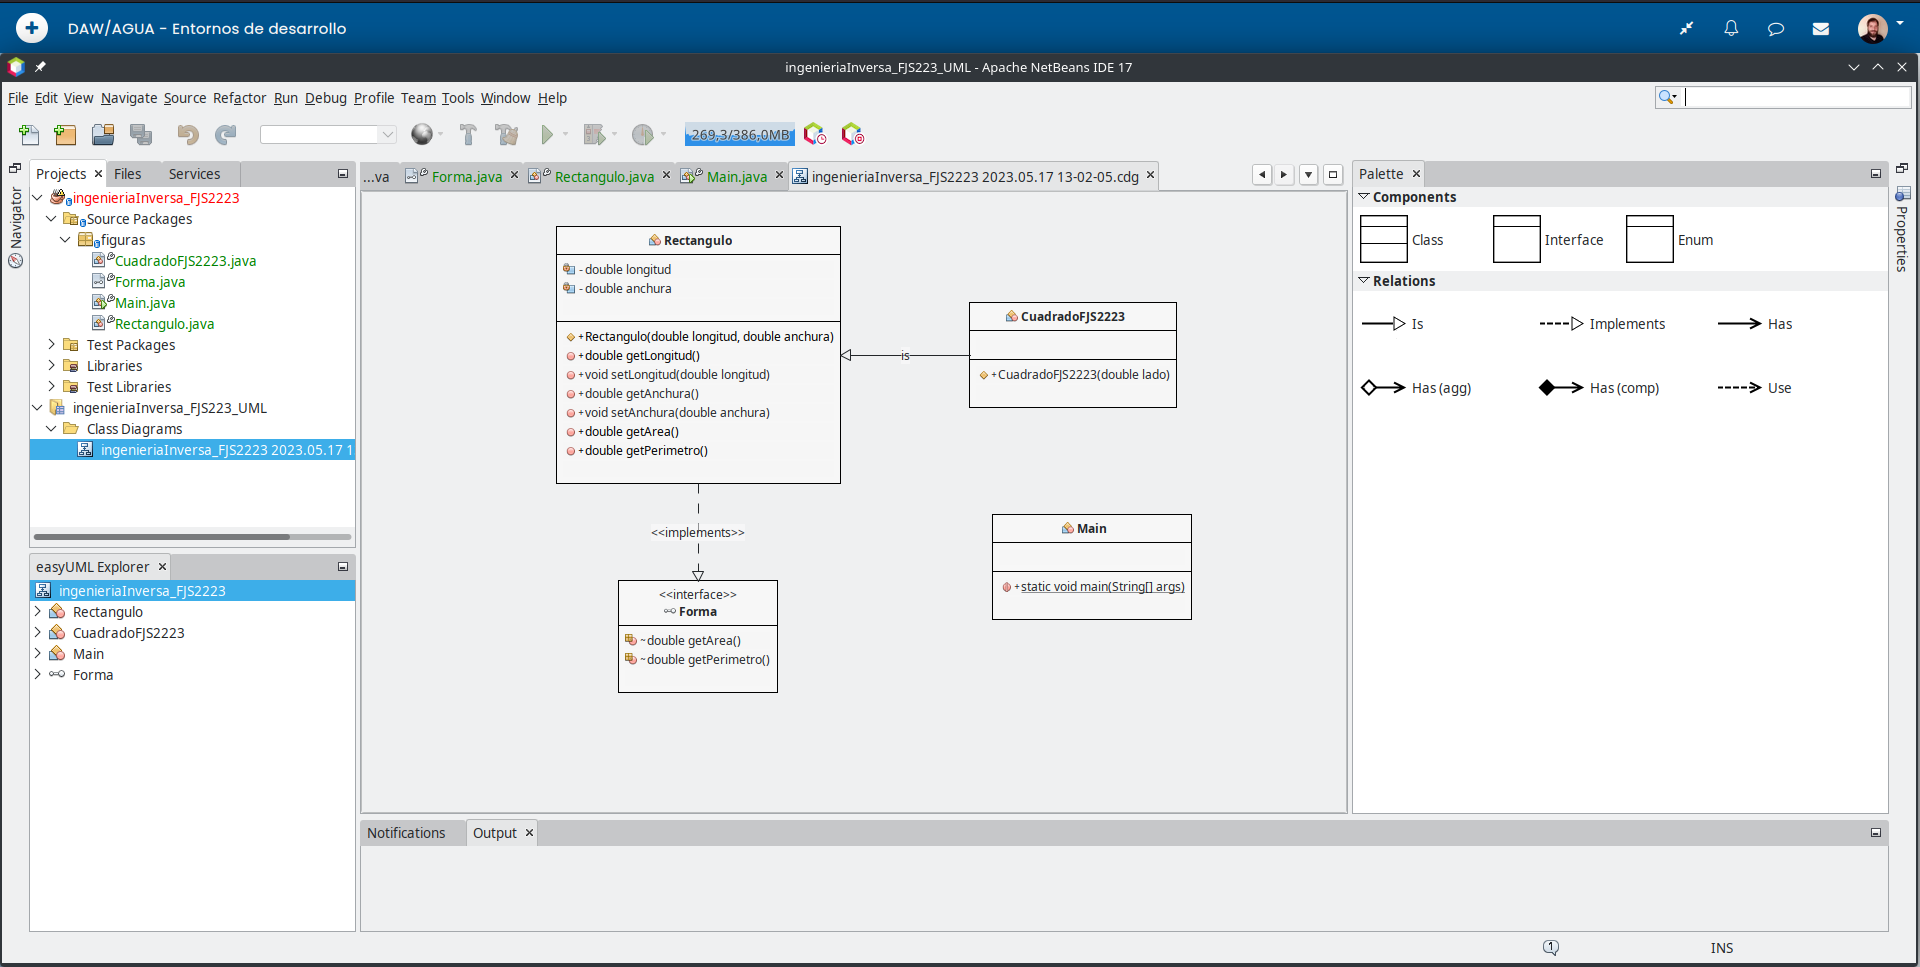
\includegraphics[scale=0.24]{inversa-4.png}
        \caption{Diagrama generado con easyUML}
    \end{figure}
\end{enumerate}

\textbf{NOTA}: en la última captura se muestra Netbeans con otro tema diferentes, ya que con el tema anterior, Dark Metal, no se apreciaban correctamente el nombre de las clases generadas con easyUML.

\section{Parte 2: Diagramas de Comportamiento}


% Bibliography
%\newpage
%\bibliography{citas}
%\bibliographystyle{unsrt}

\end{document}